% !TEX root = ../../main.tex


\begin{figure}[!htb]
\centering
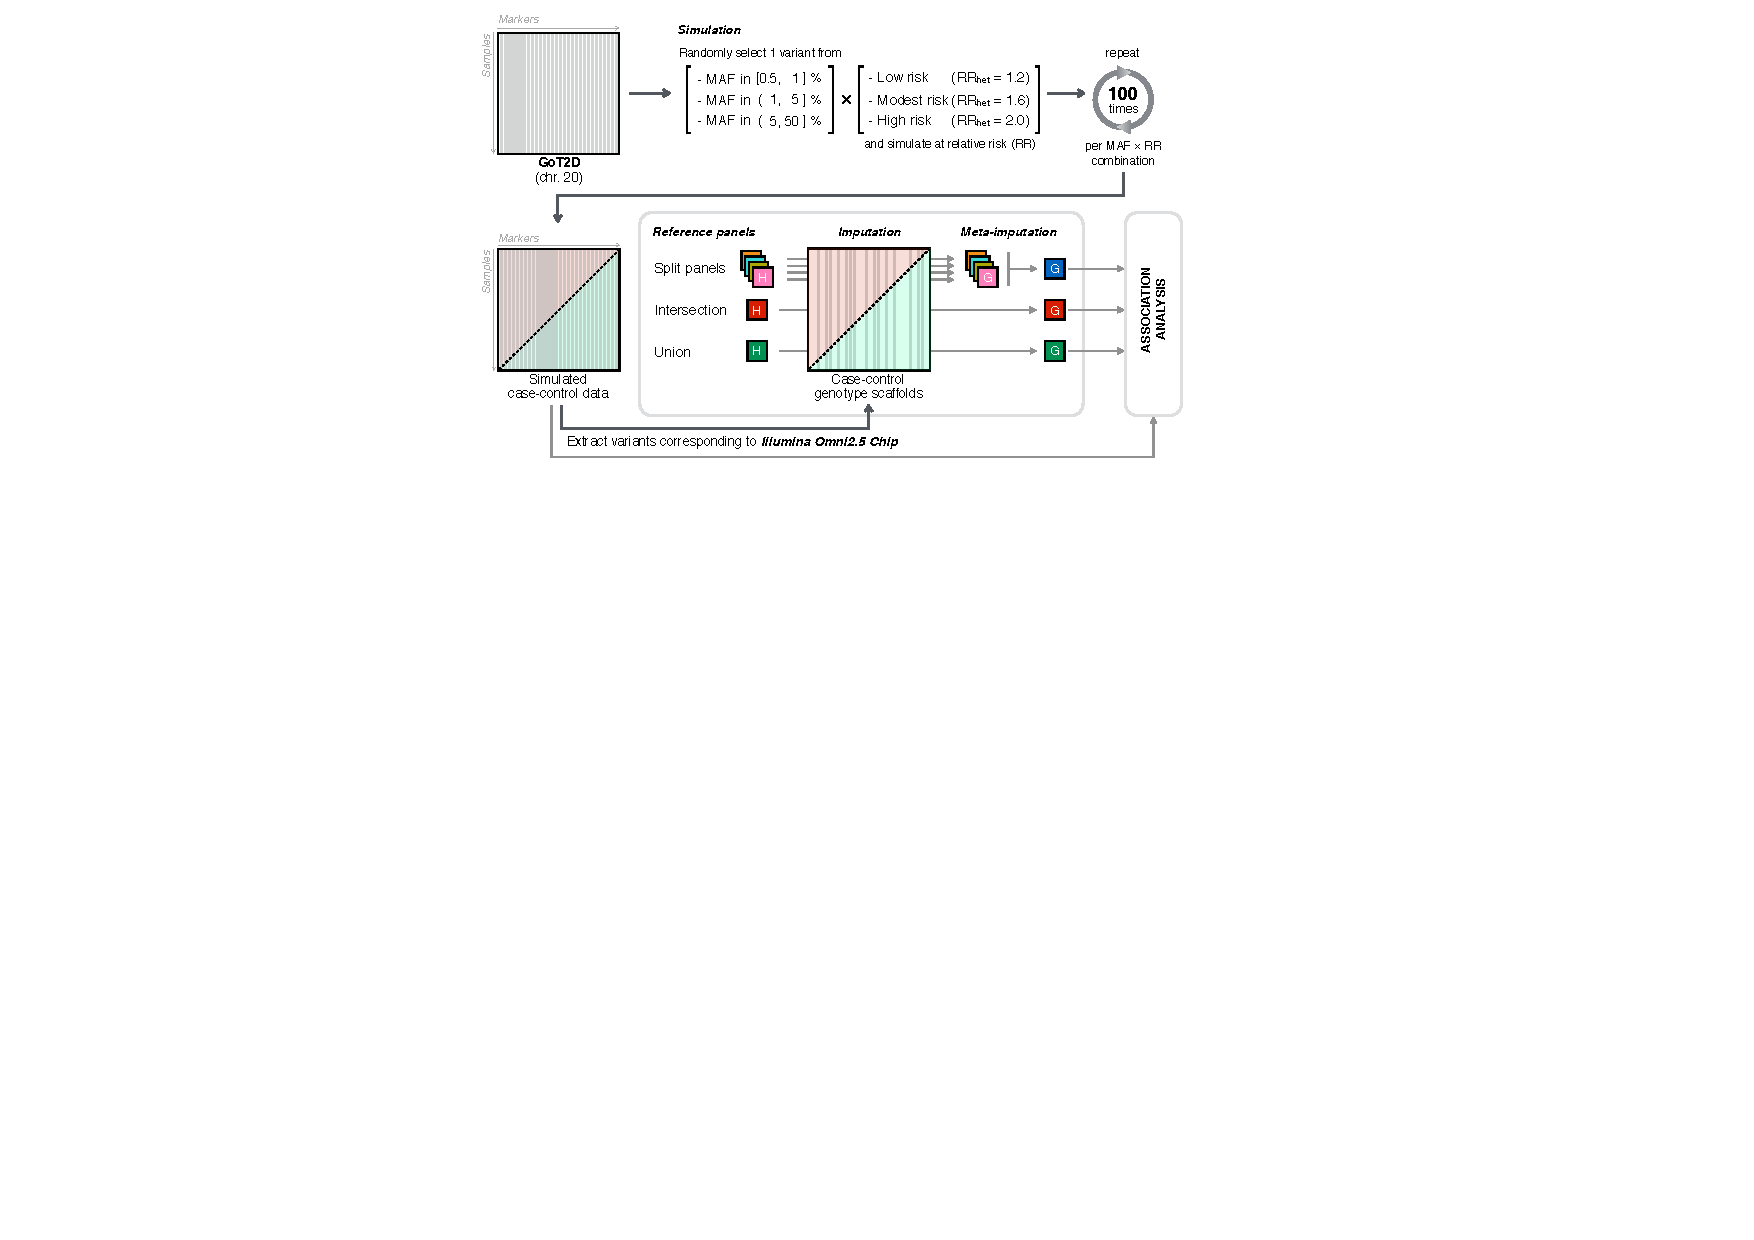
\includegraphics[width=0.9\textwidth]{./img/ch2/info_design_power}
\Caption{Illustration of the simulation process}
{Meta-imputation was assessed in terms of statistical power to detect significant risk association signals in a series of simulated case-control experiments.
The \gls{got2d} dataset was used as a template for simulations using \texttt{HAPGEN} \citep{Su:2011km}, where \n{1} variant was randomly selected within \n{1} of \n{3} defined \gls{maf} intervals.
The selected variant was then simulated to act as a causal disease variant in the simulated case-control dataset, where relative risk ($RR_{het}$) was defined according to \n{1} of \n{3} defined risk categories.
In total, \n{100} replicate simulations were conducted per combination of \gls{maf} interval and risk category (per scenario).
Simulated data were used to extract a genotype scaffold into which available reference panels were imputed, followed by meta-imputation of imputed datasets.
Imputed and meta-imputed datasets were then subjected to association analysis, including the simulated (not imputed) datasets for comparison.}
{fig:info_design_power}
\end{figure}
